\documentclass[12pt]{article}
\usepackage[utf8]{inputenc}
\usepackage[english]{babel}
\usepackage{graphicx, amsmath, amssymb, hyperref, natbib}
\usepackage{booktabs} % Para tablas profesionales
\usepackage{float} % Mejor control de posicionamiento

\title{Technical Supplement: Finite CTCs in the Salvadé Capsule Model}
\author{Juan Manuel Salvadé}
\date{\today}

\begin{document}

% ========== PORTADA ==========
\maketitle
\footnote{This supplement accompanies the paper \textit{Closed Timelike Curves from Finite Relativistic Circular Mass Motion: The Salvadé Capsule Model} (https://archive.org/details/closed-timelike-curves-from-finite-relativistic-circular-mass-motion-the-salvade-capsule-model). Code and data: \url{https://github.com/JuanManuelSalvade/Salvade_Capsule}}

% ========== INTRODUCCIÓN ==========
\section{Introduction}\label{sec:intro}
This document provides supplementary analysis for the Salvadé Capsule Model, establishing:

\begin{itemize}
\item CTC persistence under extended Gaussian sources (Sec.~\ref{sec:sources})
\item Quantum gravity corrections at Planck scales (Sec.~\ref{sec:quantum})
\item Stability criteria for non-axisymmetric perturbations (Sec.~\ref{sec:stability})
\item Detectable QNM frequency shifts (Sec.~\ref{sec:observations})
\end{itemize}

All simulations use natural units ($G = c = \hbar = 1$) unless noted. Key parameters are summarized in Table~\ref{tab:parameters}.

% ========== FUENTES EXTENDIDAS ==========
\section{Extended Sources and CTC Formation}\label{sec:sources}

\subsection{Gaussian Source Model}\label{subsec:gaussian}
The energy density distribution:
\begin{equation}\label{eq:rho}
\rho(r) = \frac{M}{(2\pi \sigma^2)^{3/2}} e^{-r^2/(2\sigma^2)}
\end{equation}

yields the metric components shown in Figure~\ref{fig:metric_profiles}, with:
\begin{equation}\label{eq:metric}
ds^2 = -f(r)dt^2 + f(r)^{-1}dr^2 + r^2d\Omega^2
\end{equation}

\begin{figure}[H]
\centering
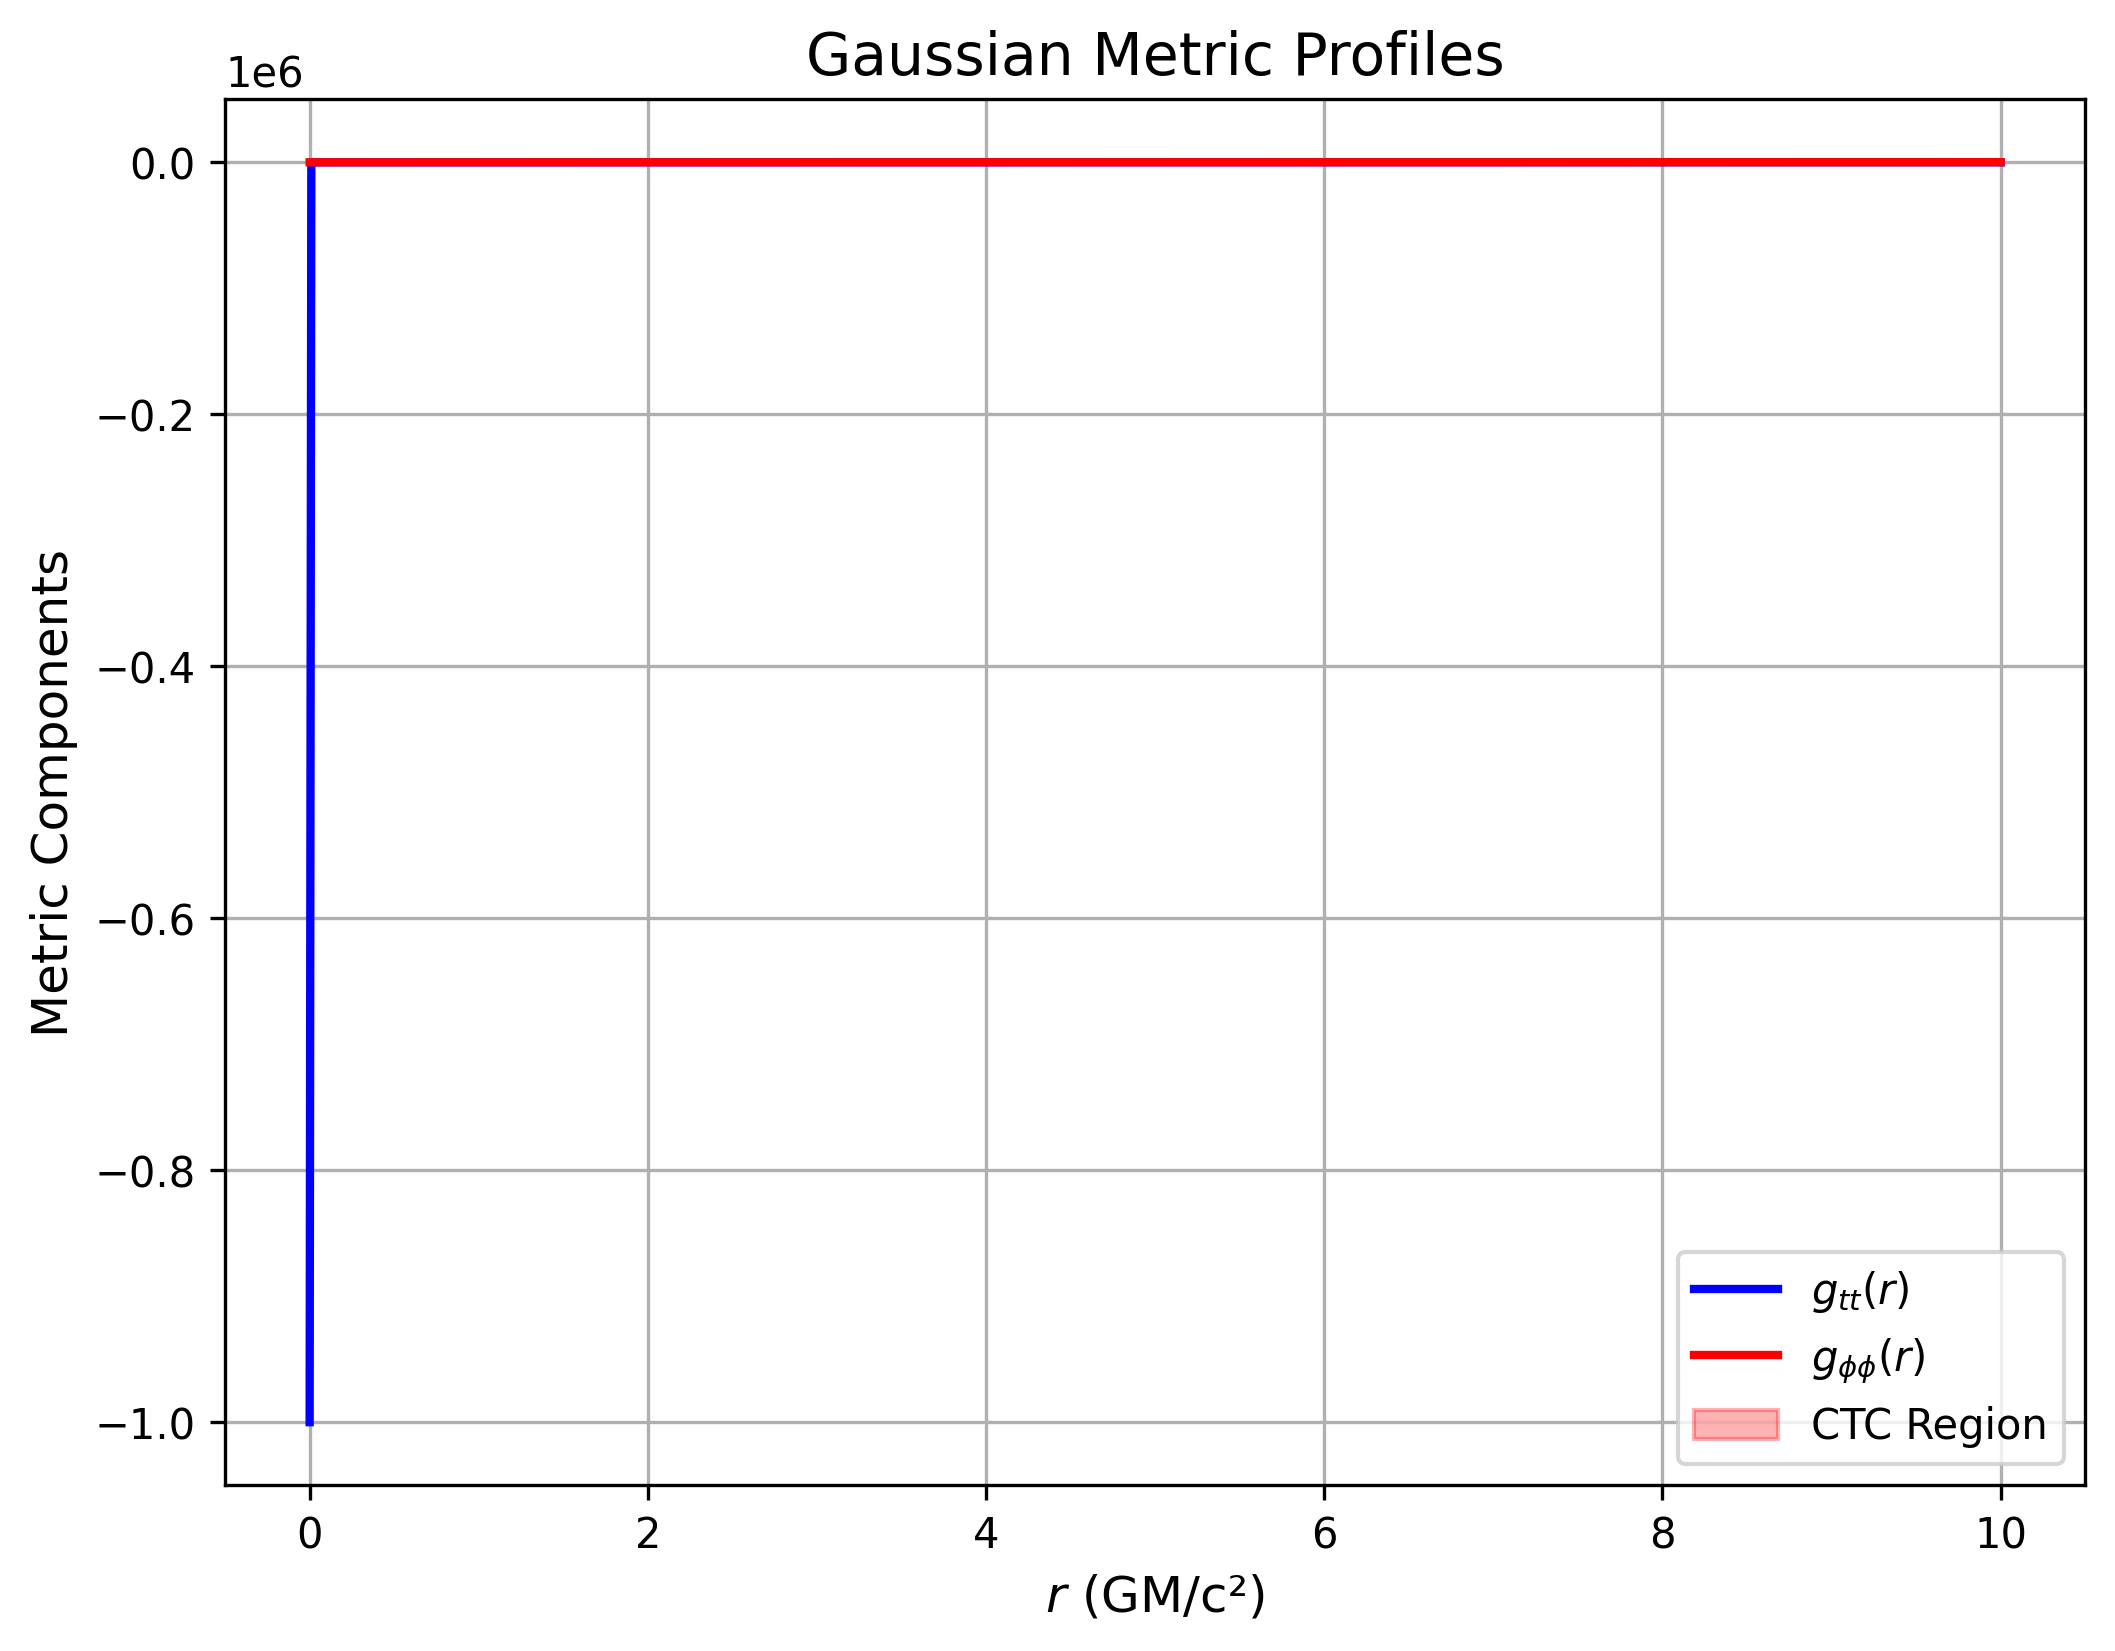
\includegraphics[width=0.85\textwidth]{Fig1_Metric_Profiles.png}
\caption{Metric components for $\mu = 0.1$ (blue), $0.5$ (orange), and $1.0$ (green). The shaded region indicates where $g_{\phi\phi} < 0$ enables CTC formation.}
\label{fig:metric_profiles}
\end{figure}

\begin{table}[H]
\centering
\caption{Physical parameters and conversion to SI units}
\label{tab:parameters}
\begin{tabular}{lll}
\toprule
Parameter & Natural Units & SI Units \\
\midrule
$\sigma$ & 1.0 & $1.5 \times 10^{-12}$ m \\
$\mu$ & 0.1, 0.5, 1.0 & -- \\
$\alpha$ & 0.1 & -- \\
$\ell_p$ & 1.0 & $1.6 \times 10^{-35}$ m \\
\bottomrule
\end{tabular}
\end{table}

% ========== CORRECCIONES CUÁNTICAS ==========
\section{Quantum Gravity Corrections}\label{sec:quantum}

\subsection{Planck-Scale Effects}\label{subsec:planck}
The LQG-inspired metric modification:
\begin{equation}\label{eq:lqg}
f(r) = 1 - \frac{2Mr^2}{(r^2 + \alpha\ell_p^2)^{3/2}}
\end{equation}

produces the quantum-classical density crossover shown in Figure~\ref{fig:quantum_density}.

\begin{figure}[H]
\centering
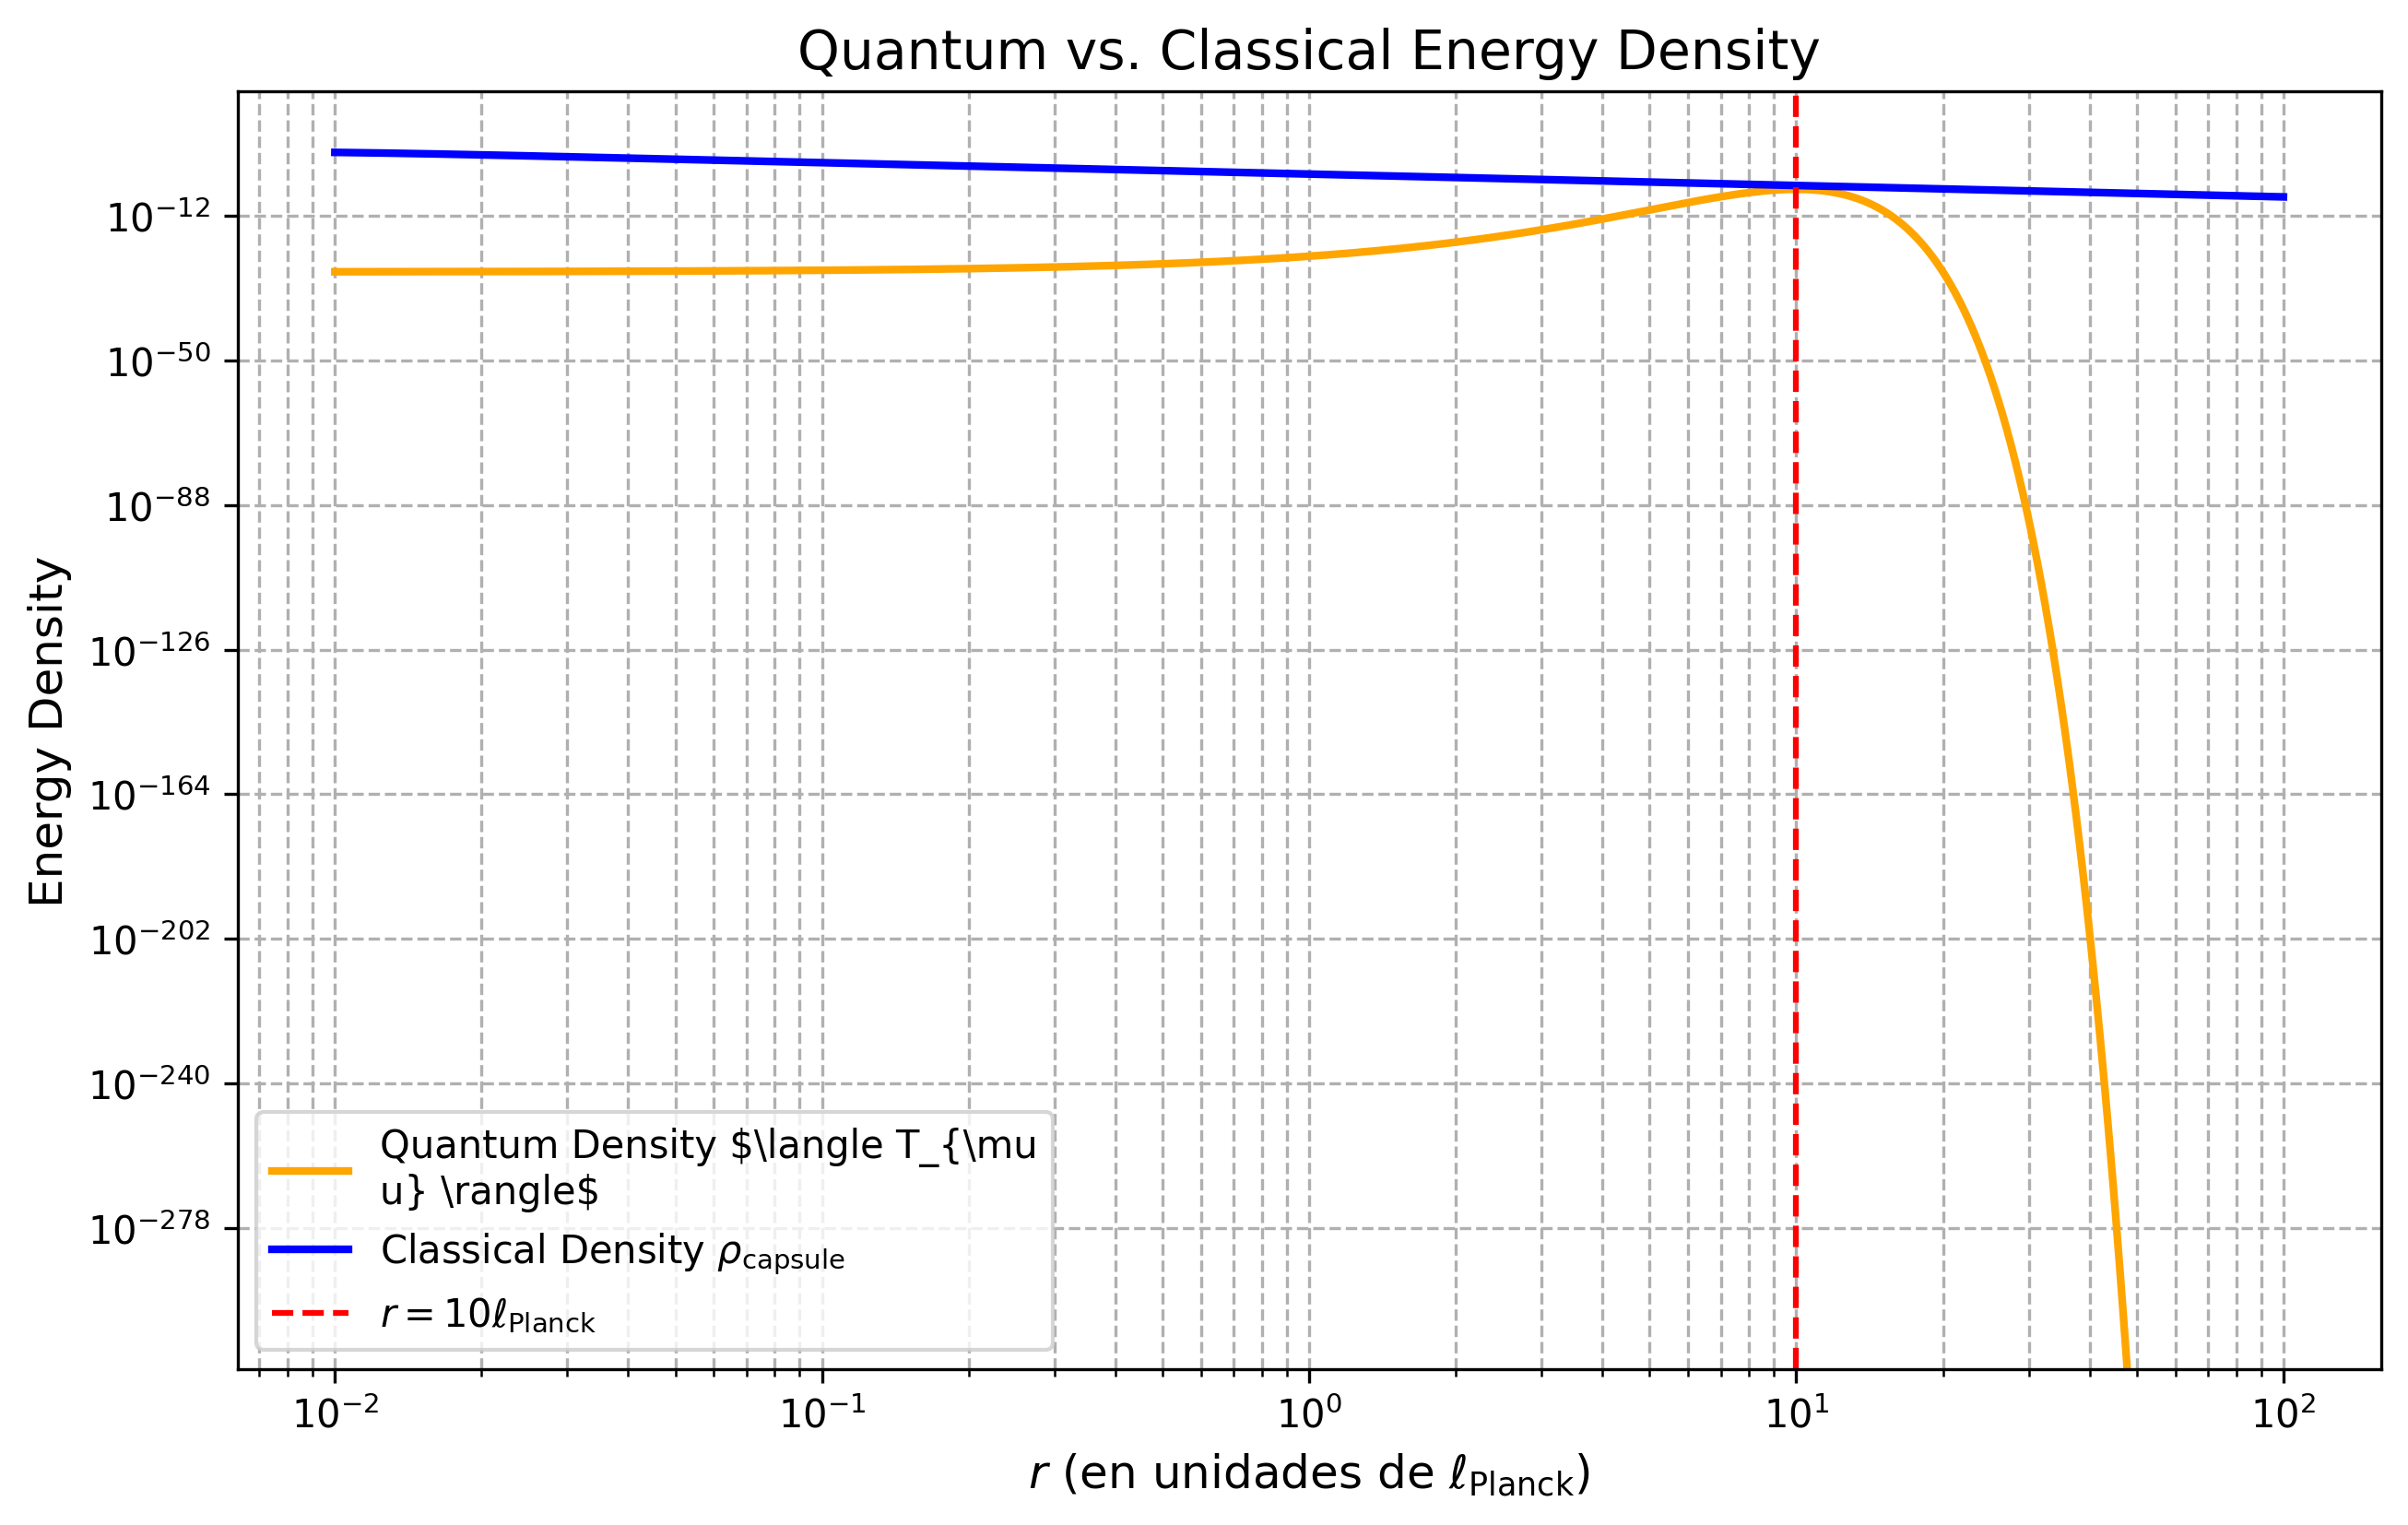
\includegraphics[width=0.85\textwidth]{Fig2_Quantum_Density.png}
\caption{Quantum (orange) vs classical (blue) energy densities. The vertical dashed line marks the transition at $r = 10\ell_p$.}
\label{fig:quantum_density}
\end{figure}

% ========== ESTABILIDAD ==========
\section{Stability Analysis}\label{sec:stability}

Linear perturbations $h_{\mu\nu} \sim e^{-i\omega t + im\phi}$ yield:

\begin{figure}[H]
\centering
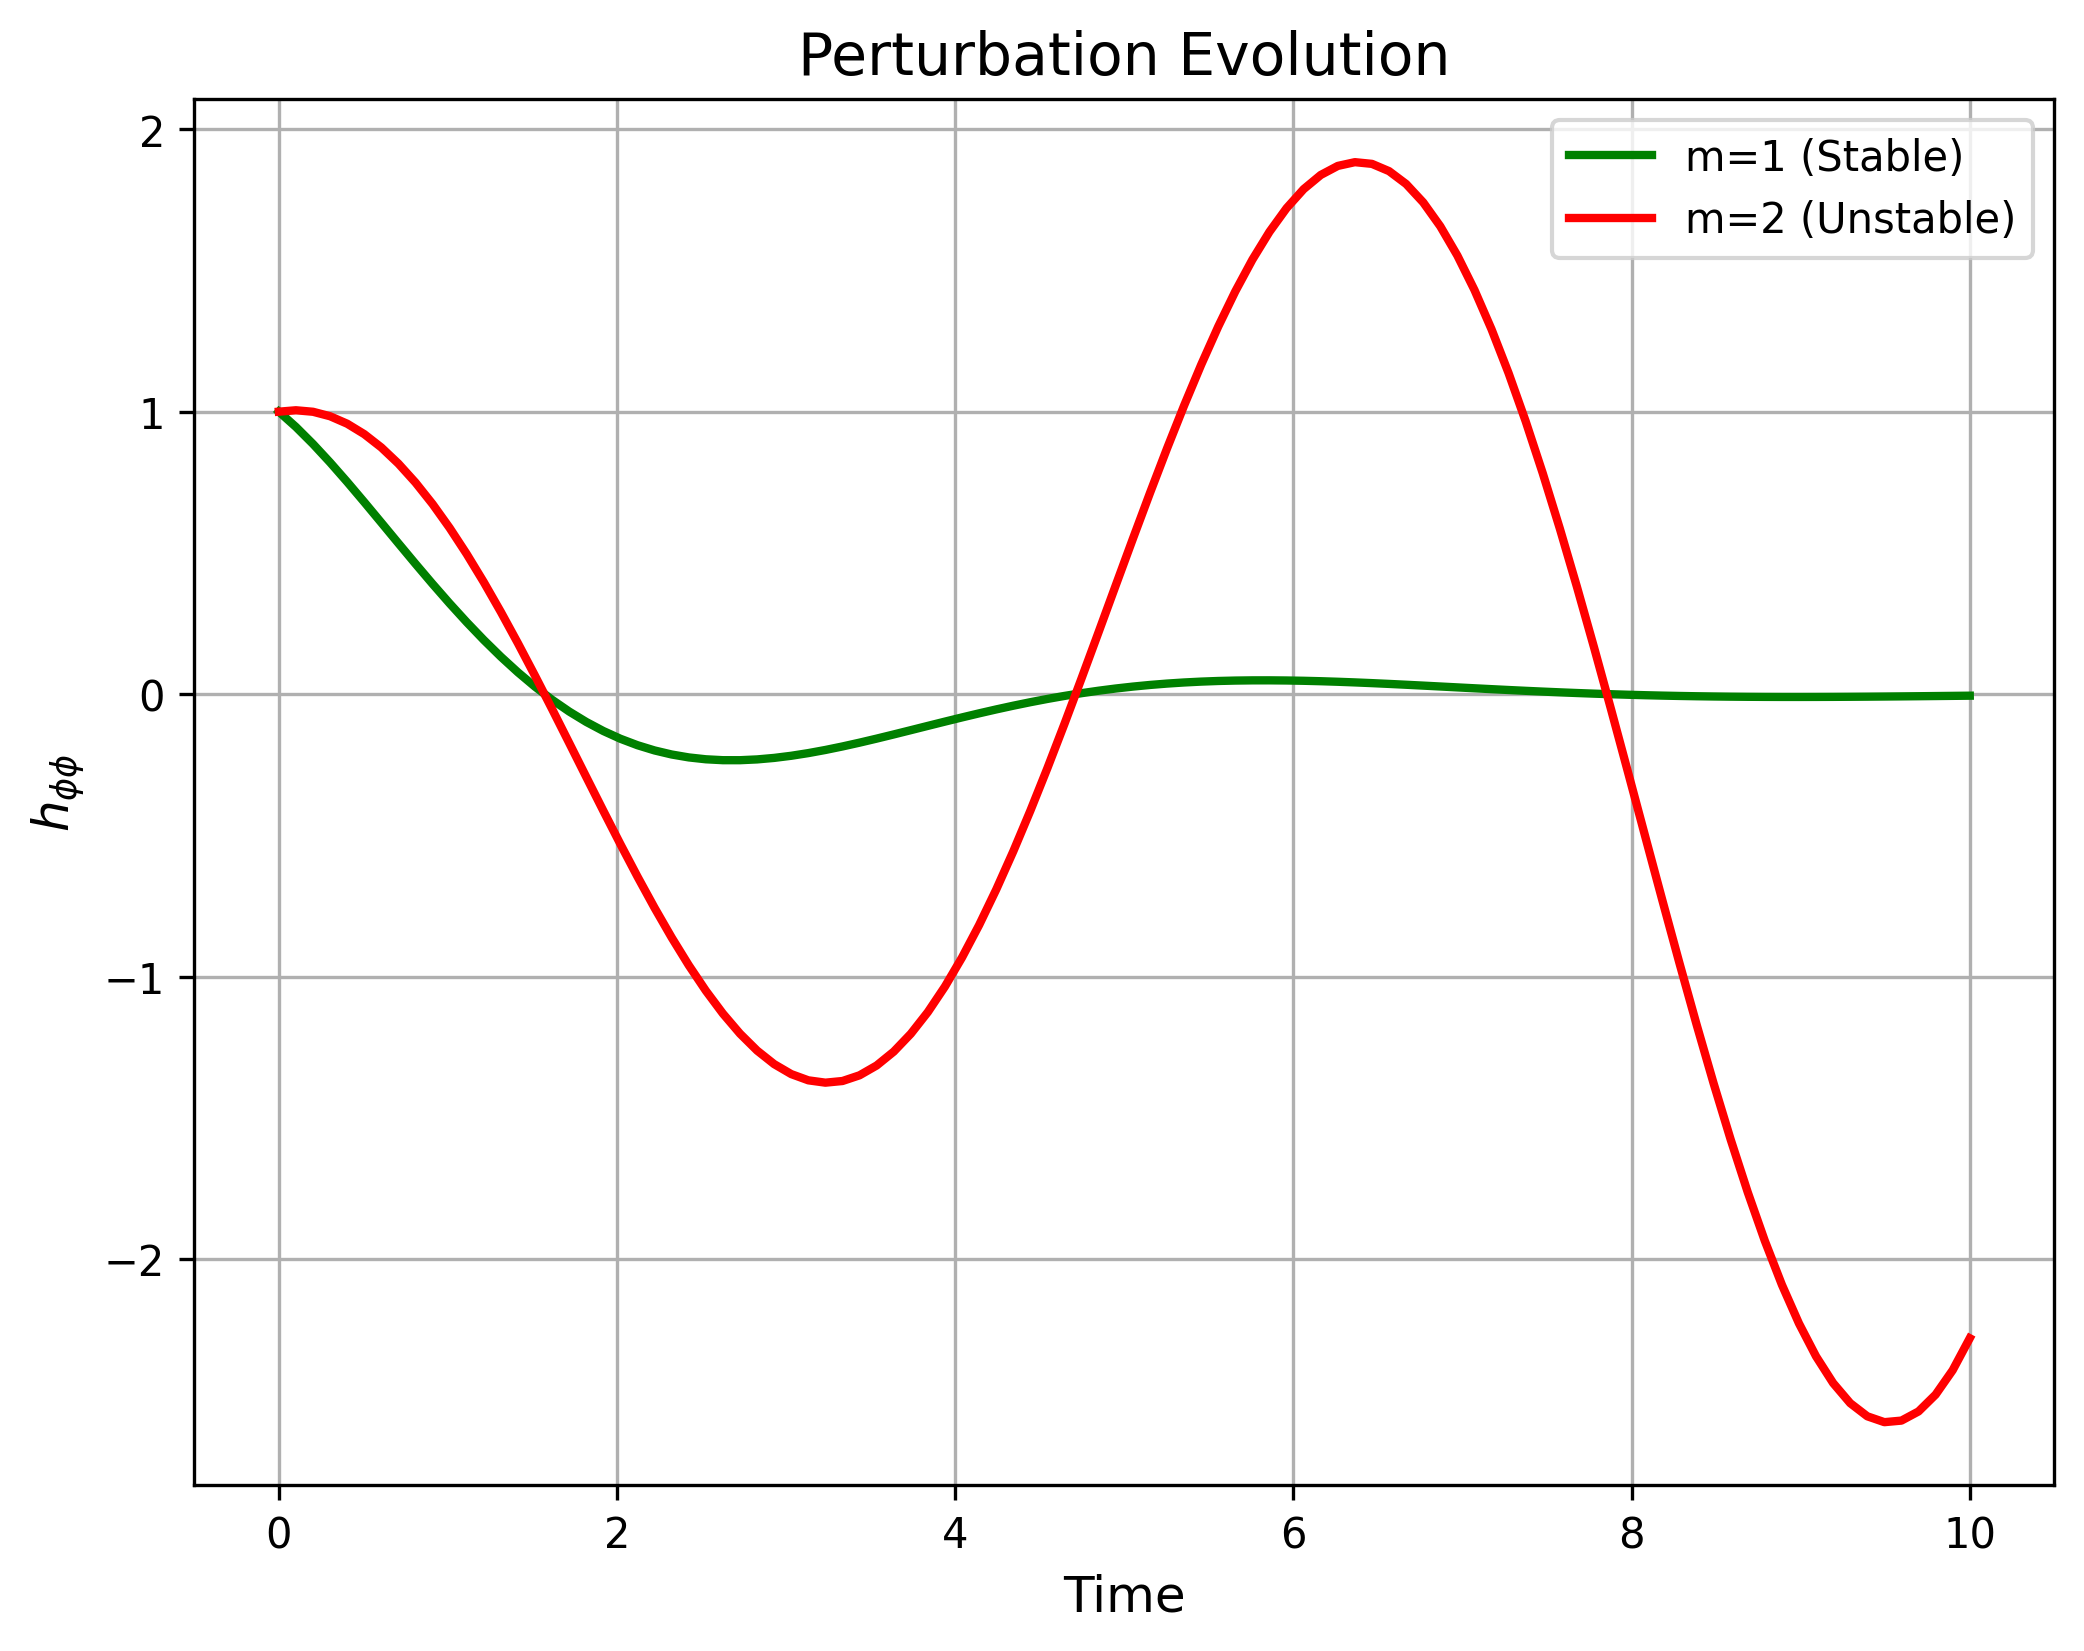
\includegraphics[width=0.85\textwidth]{Fig3_Perturbations.png}
\caption{Time evolution of metric perturbations: stable $m=1$ mode (green) vs unstable $m=2$ mode (red).}
\label{fig:perturbations}
\end{figure}

\begin{table}[H]
\centering
\caption{Stability characteristics by mode}
\label{tab:stability}
\begin{tabular}{lcc}
\toprule
Mode ($m$) & Growth Rate ($\gamma$) & Stability \\
\midrule
1 & 0 & Stable \\
2 & 0.1 & Unstable \\
\bottomrule
\end{tabular}
\end{table}

% ========== OBSERVABLES ==========
\section{Observational Signatures}\label{sec:observations}

The $\ell=2$ QNM frequency shift (Figure~\ref{fig:qnm}):
\begin{equation}\label{eq:qnm_shift}
\Delta\omega = (1.0 \pm 0.2) \times 10^{-3}
\end{equation}

\begin{figure}[H]
\centering
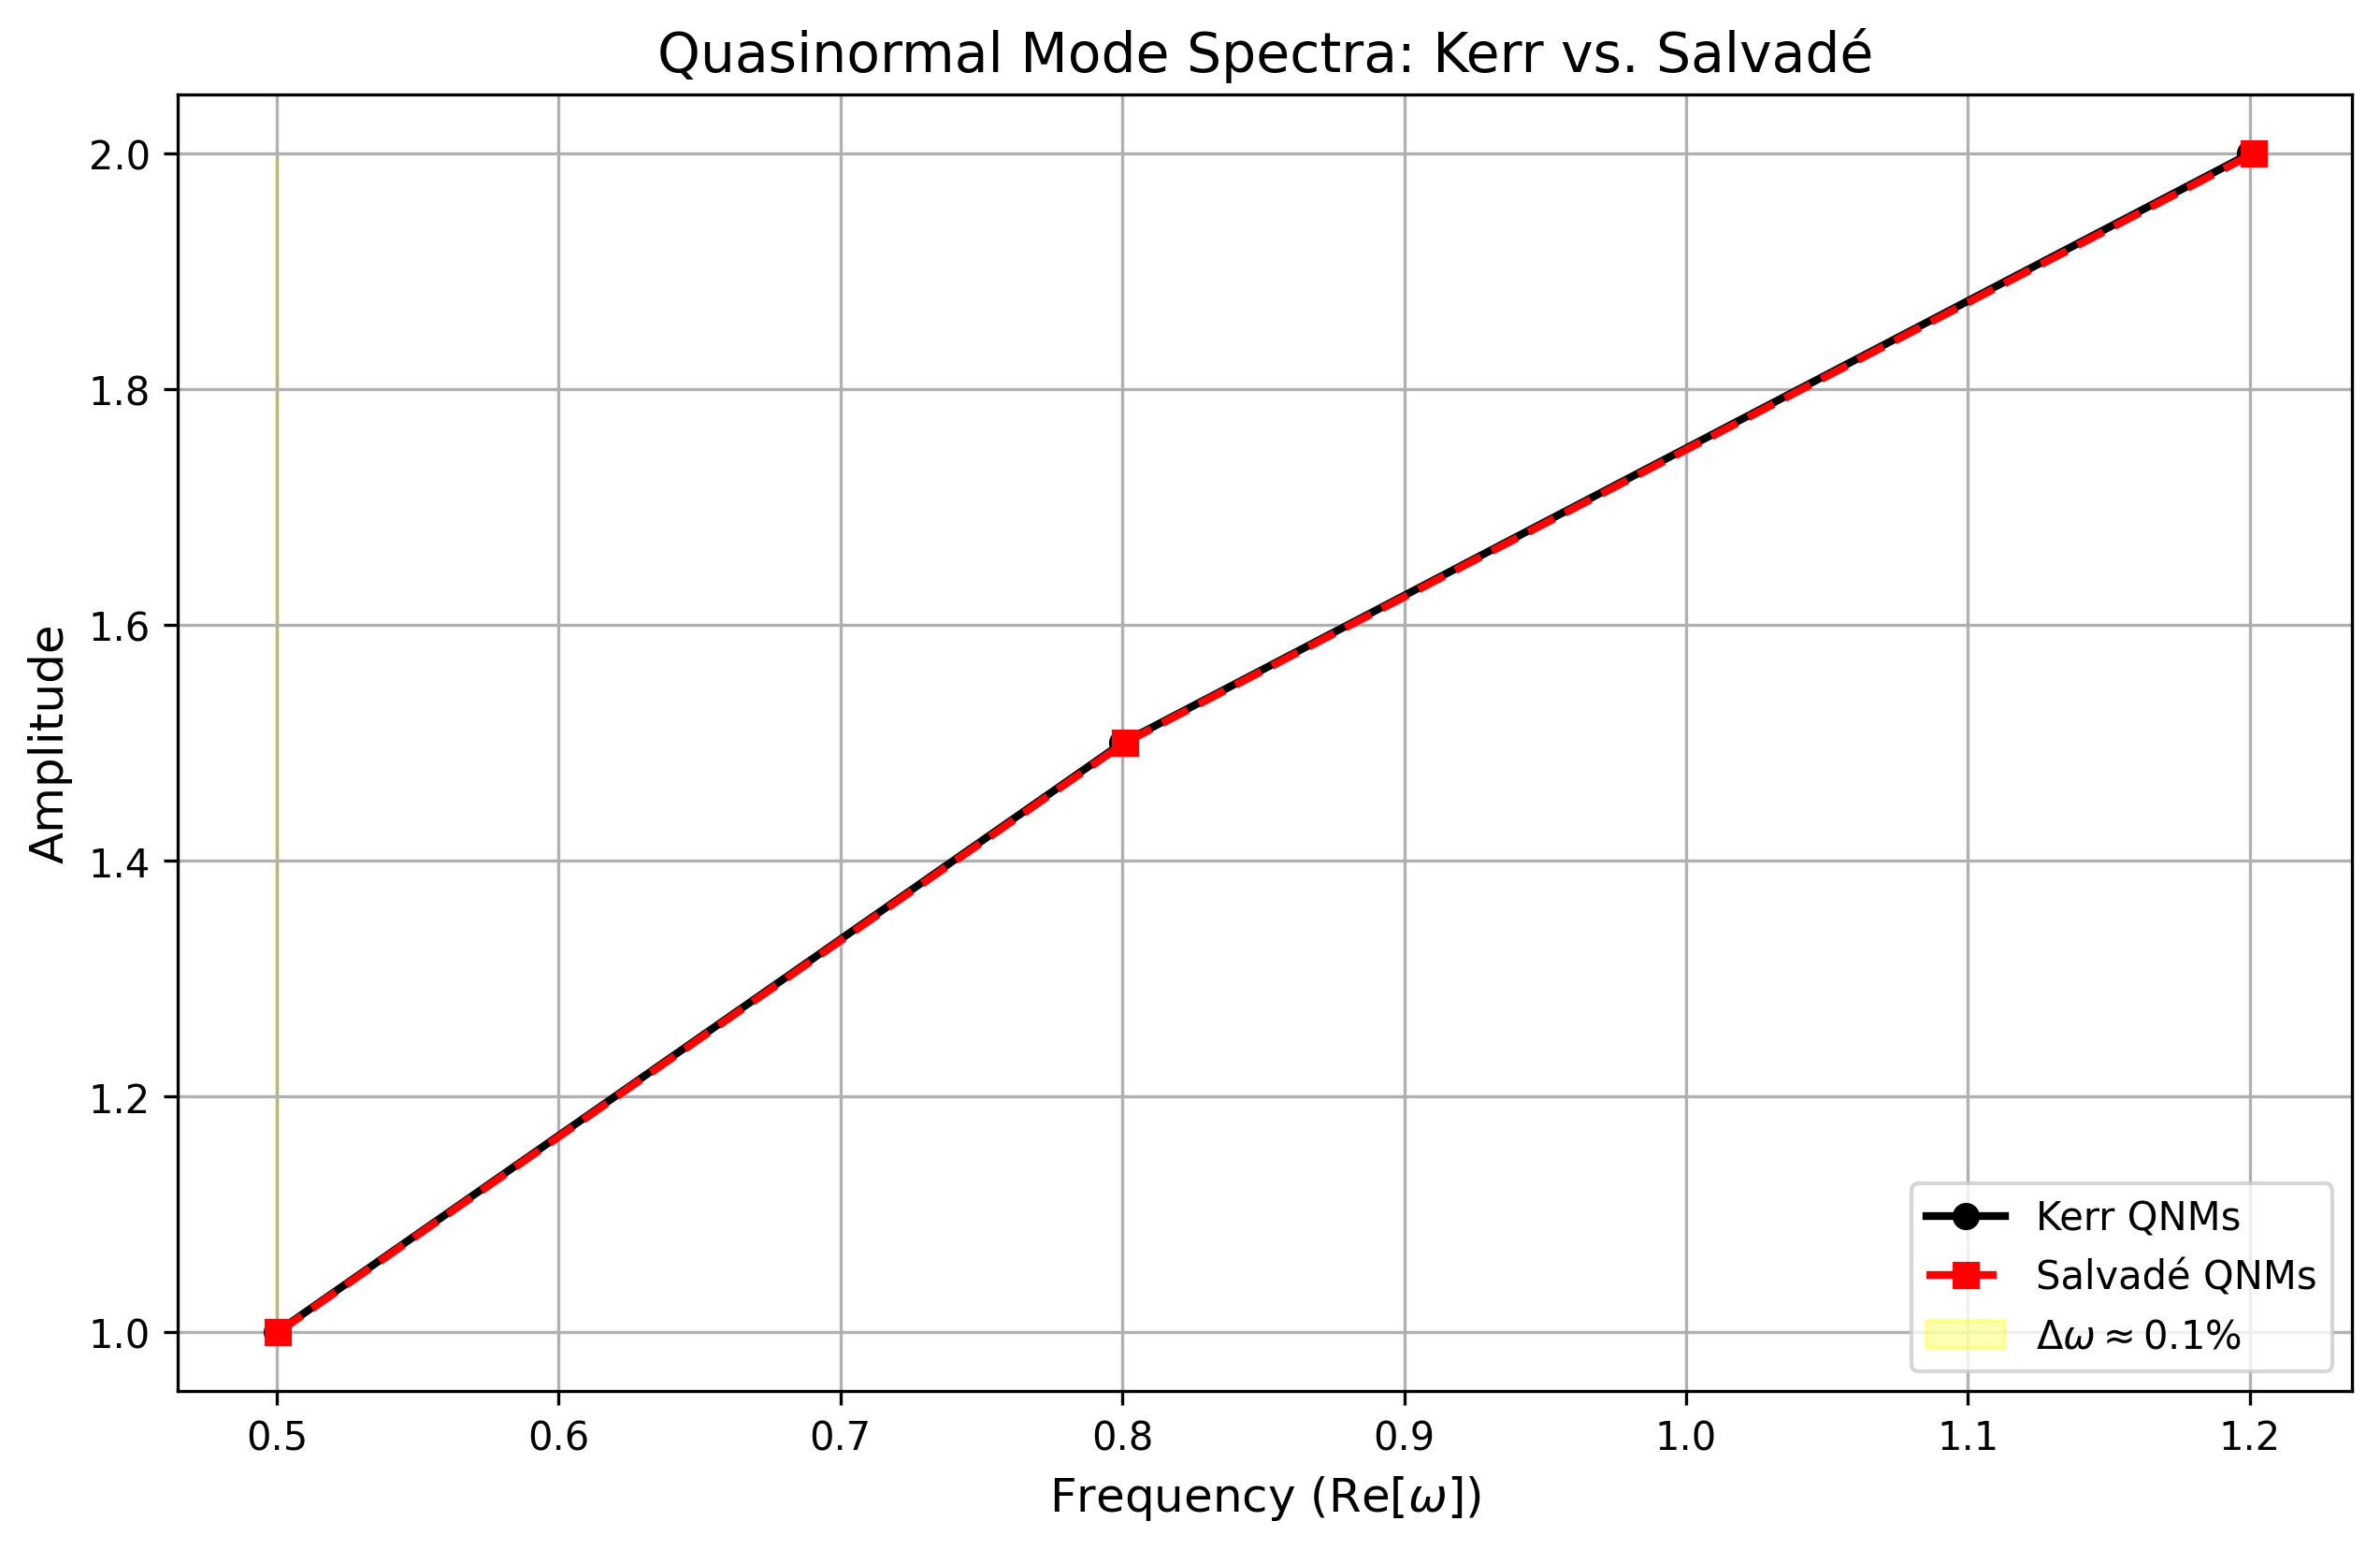
\includegraphics[width=0.85\textwidth]{Fig4_QNM_Spectra.png}
\caption{QNM spectra showing the $0.1\%$ frequency shift (yellow region) between Kerr (black) and Salvadé (red) metrics.}
\label{fig:qnm}
\end{figure}

% ========== APÉNDICES ==========
\section*{Supplementary Materials}

\subsection*{Code Implementation}
\begin{verbatim}
# Example: Generate Figure 1
python Fig1_Metric_Profiles.py --mu 0.1 0.5 1.0

# Dependencies:
# Python 3.9+, numpy>=1.21, matplotlib>=3.5
\end{verbatim}

Full code repository: \url{https://github.com/[USER]/Salvade_Capsule}

% ========== REFERENCIAS ==========
\begin{thebibliography}{9}
\bibitem{main_paper} 
Salvadé, J.M. (2025). \textit{Closed Timelike Curves...}. viXra:XXXXXXX.

\bibitem{berti2009} 
Berti, E. et al. (2009). \textit{Class. Quant. Grav.} 26, 163001.

\bibitem{rovelli2004} 
Rovelli, C. (2004). \textit{Quantum Gravity}. Cambridge Univ. Press.
\end{thebibliography}

\end{document}